\chapter{System Models}

\section{Scenarios}
The scenarios are based on Node.js based web applications on a server running root and rootJS\\

Web viewer launches and provides a GUI to its end user	\\
Web viewer requests data for visualization by calling rootJS\\
\indent	Node.js invokes ROOT I/O operations\\
\indent \indent		ROOT loads data and provides raw visualization data\\
\indent	Node.js serializes data and streams it to the web viewer\\
Web viewer receives data and renders it in the browser\\
\section{Use Cases}

\pagebreak[4]

\section{Object Models}
\begin{figure}[htb]
	\centering
	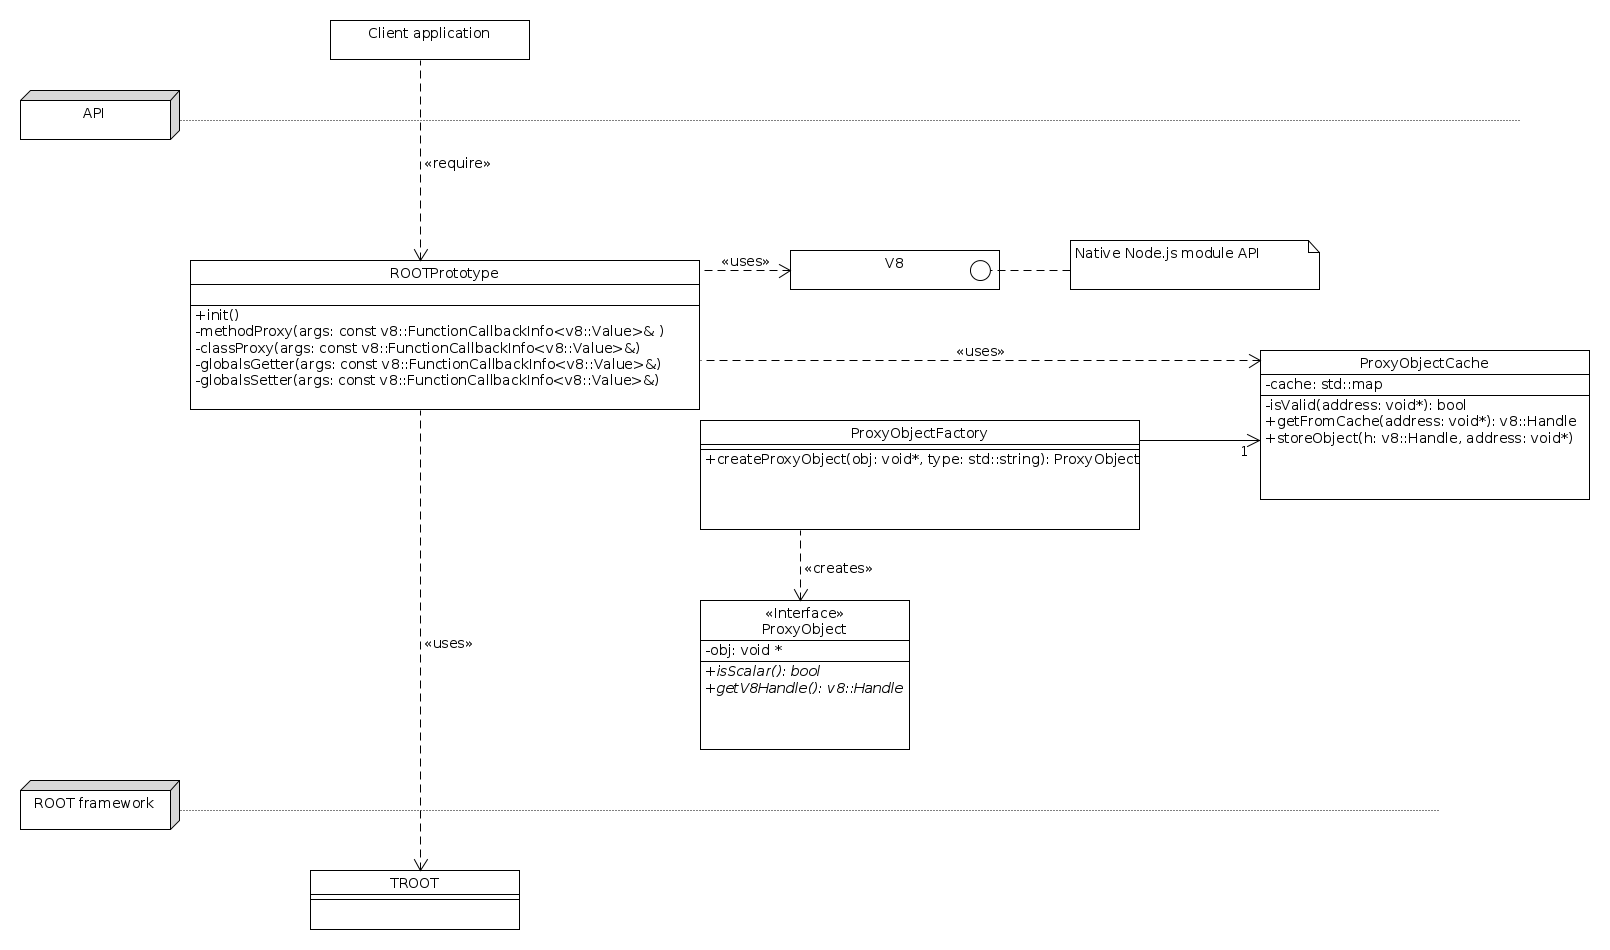
\includegraphics[width=18cm]{./latex/resources/architecture.png}
	\caption{basic architecture draft}
\end{figure}

\pagebreak[4]

\section{Dynamic Models}
\begin{figure}[htb]
	\centering
	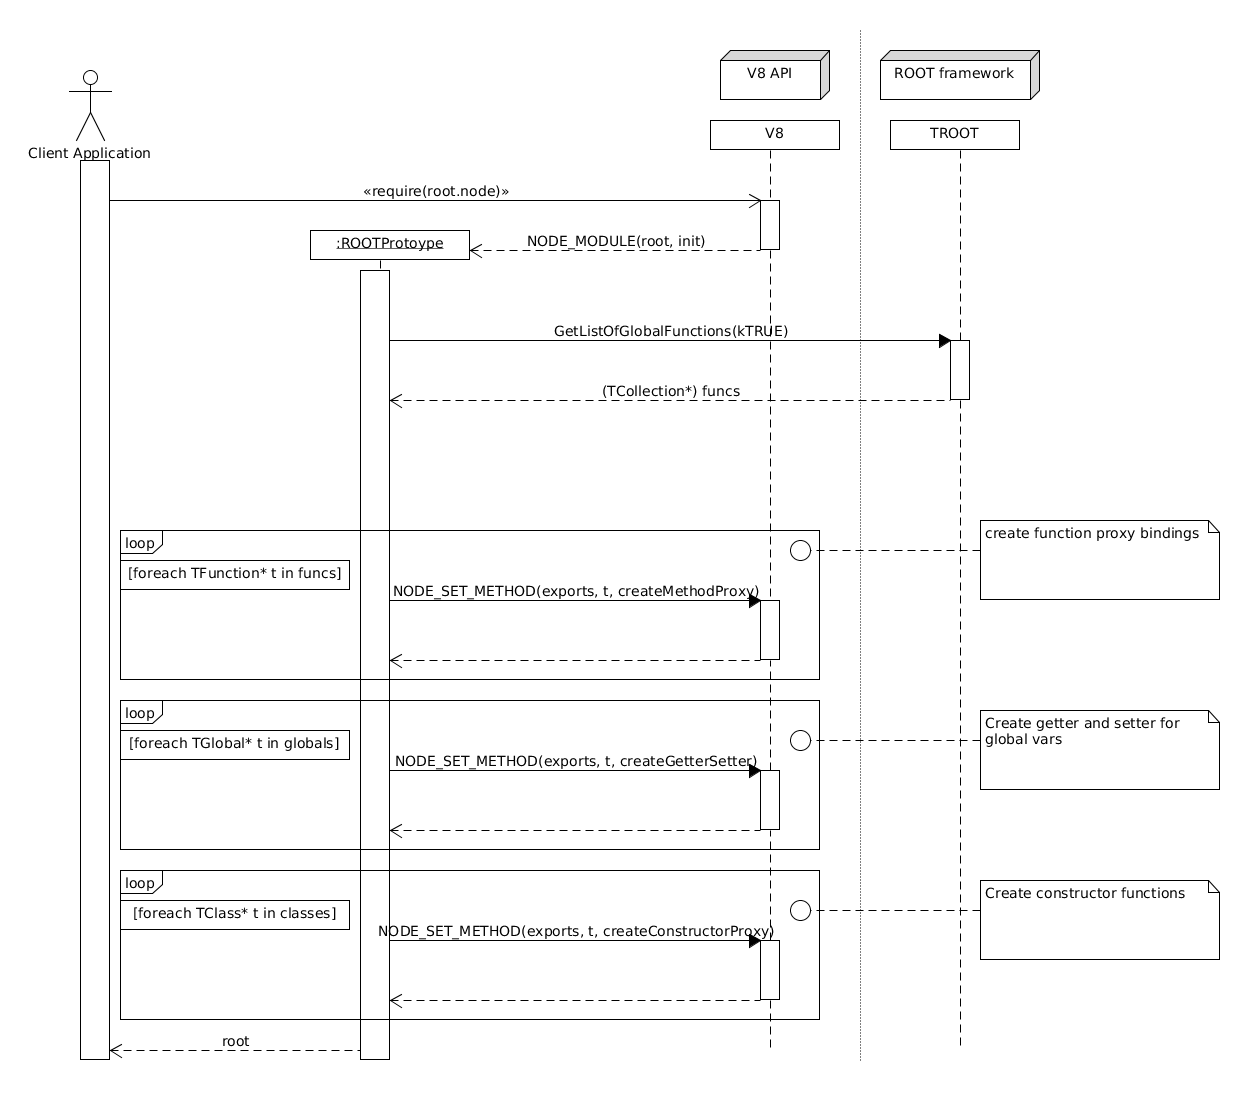
\includegraphics[width=18cm]{./latex/resources/startupSequence.png}
	\caption{startup sequence}
\end{figure}
